\usepackage[english]{babel}
\usepackage[T1]{fontenc}
\usepackage[utf8]{inputenc}
\usepackage{graphicx}
\usepackage{listings}
\usepackage{amsmath}
\usepackage{amssymb}
%\usepackage{amsthm}
\usepackage{ae,aecompl}
\usepackage{fix-cm}

\usetheme{Goettingen}
%\usetheme{Singapore}

\beamertemplatenavigationsymbolsempty
\beamertemplatetextbibitems

\newcommand{\leftexp}[2]{{\vphantom{#2}}^{#1}{#2}}


\title{Face and edge transitive tilings in three dimensional non-Euclidean
spaces}
\author{Boróczki, Lajos}
\date{Budapest, 11-13 June 2012 \\{\tiny Workshop of the BME Graduate School of
Mathematics and Computer Science}}

\begin{document}

\begin{frame}
  \maketitle
\end{frame}

\begin{frame}
  \mode<presentation>{\frametitle{Outline}}
  \tableofcontents
\end{frame}
\newpage

\section{Abstract}
\begin{frame}
  \tiny
Workshop of the BME Graduate School of
Mathematics and Computer Science\\
Budapest, 11-13 June 2012
\vfill
\normalsize
\begin{center} 
  Face and edge transitive tilings in three dimensional non-Euclidean spaces
\end{center}

\vfill
\tiny
\textbf{BORÓCZKI, Lajos}\\
Budapest University of Technology and Economics, MI Department of Geometry\\
E-mail: boroczki.lajos@gmail.com\\
\vfill

http://www.math.bme.hu/~boroczki
\vfill

\tiny
\textbf{Abstract.}  Any tiling, generated by a crystallographic group with
compact fundamental domain, can be represented by a diagram and a matrix valued
function, based on their barycentric subdivision and the adjacency relations
between the orbits and the particular simplices. The representation is called
the D-symbol of a tiling in honour of Delone, Delaney and Dress. The
representation is easily adaptable to computer programs.
\vfill

Both face and edge transitive tilings are special tilings, which have only 1
face or edge orbit respectively in the crystallographic group. (Our fundamental
domain doesn't have to be the smallest possible, it can have inner symmetries.)
It's easy to prove that there are finitely many possible diagrams in these
cases, so enumerating all of them in every possible geometry seems possible.
\vfill

The problem in the non-Euclidean planes (E. Molnár with  Z.  Lu\u{c}i\'{c} and
M. Stojanovi\'{c} (1994)) and in the space $E^3$ (E. Molnár with A.W.M. Dress
and D.H. Huson (1993)) is already solved.
\vfill

We can enumerate tilings with at most 18 simplex-orbits (out of 24). Three
dimensional tilings induce some two dimensional tilings around the vertices of
the simplices and between any two partition of the simplex-vertices. These can
be examined by a simple formula, which gives us finitely many possible matrix
valued functions for every diagram to investigate.
\vfill

Based on the Thurston-theorem there are 8 possible geometries.  There exists at
least 4 proof of the theorem but none of them is constructive. Based on our
method it would be easier to find a tiling which does not fit in any of the 8
geometries; but inspecting the tilings we can possibly move forward to a
constructive proof of the theorem.
\vfill

But there are some more problems to solve first: we have to find the possible
splittings in a D-symbol (which corresponds to tori in Thurston's notation)
and we have to be able to tell the signature of the projective space of the
tiling of a primitive D-symbol.
\vfill

The results discussed above are supported by the grant TÁMOP -
4.2.2.B-10/1--2010-0009.

\end{frame}

\section{D-symbols}
\begin{frame}
  \frametitle{D-symbol, an algebraic way to describe tilings}
  \begin{itemize}
    \item Based on the baricentric subdivision of an $n$-dimensional tiling and its fundamental
      domain \mode<article>{one can define the placement of the consisting
      simplices. In a baricentric subdivision the vertices can be indexed with
      the dimension of its facet. Our definition of a fundamental domain allows
      inner symmetries.}
    \item Structure:
      \begin{itemize}
        \item D-diagram: $(n+1)$ colored graph, which represents adjacencies of
          simplex-orbits
        \item Matrix function on simplex orbits, which represents the number of
          simplices (not orbits) around a $(n-2)$-dimensional edge
      \end{itemize}
    \item Constraints:
      \begin{itemize}
        \item Compatibility between the diagram and the matrix function
        \item Compatibility with baricentric subdivision
        \item Lower dimensional constraints
      \end{itemize}
    \item Every "nice" tiling has a corresponding D-symbol which is unambigous
      up to permutation \mode<article>{"Nice" tilings are the ones, whose
      baricentric subdivision has finitely many simplex-orbits and does not have
      ideal simplex-vertices except for 0-center or 3-center vertices.}
  \end{itemize}
\end{frame}

\subsection{Face/edge transitivity}
\begin{frame}
  \frametitle{Face and edge transitive D-symbols, duality}
  \mode<article>{Only in 3 dimensions.}
  \begin{itemize}
    \item A face transitive tiling has a fundamental domain with only $1$ orbit
      of faces
    \item An edge transitive tiling has a fundamental domain with only $1$ orbit
      of edges
    \item Duality between face and edge transitive tilings\mode<article>{If we
      switch the $k$th color with the $n-k$th color, and switch the matrix
      function's rows and columns respectively we get the dual D-symbol. Same
      tiling, dual fundamental domain.}
    \item A face/edge transitive D-diagram remains connected if we cancel the
      $2$nd/$1$st color \mode<article>{respectively.}
    \item A face transitive tiling's faces can be at most hexagons limiting
      possible simplex-orbits to at most $24$ \mode<article>{on both types of
      tilings. That means there can only be finitely many D-diagrams, so we can
      enumerate them.} 
  \end{itemize}
\end{frame}

\subsection{Example}
\begin{frame}
  \frametitle{Example}
  Simple edge transitive example based on the symmetry breaking of the cube tiling of
  $\mathbb{E}^3$:
  \mode<article>{figure \ref{abra:example1}. As adjacency relations are defined
  for every simplex orbit, we can skip showing the loops which map the orbits
  mirroring to a plane.}
  \begin{figure}
    \mode<article>{\caption{\label{abra:example1} Red:1, blue:2, green:3,
    yellow:4}}
    \center
    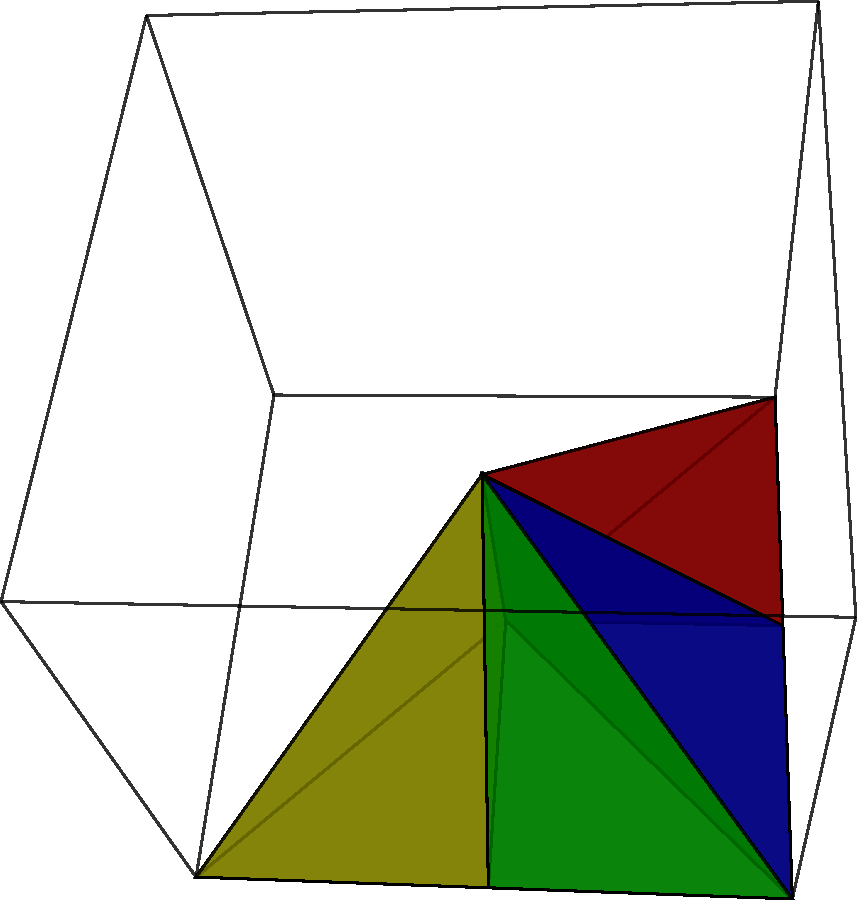
\includegraphics[width=0.3\textwidth]{d3c4_7_1.pdf}
    \hfill
    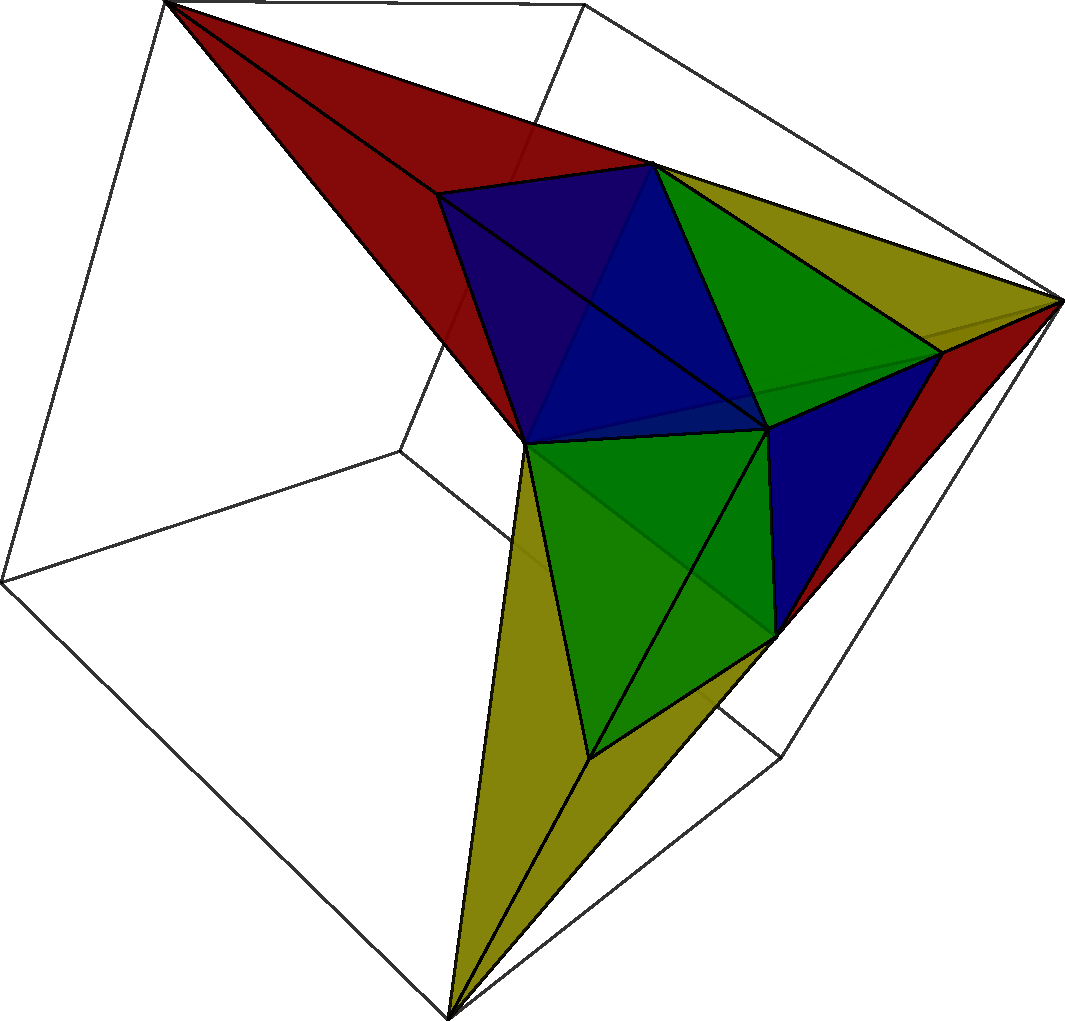
\includegraphics[width=0.3\textwidth]{d3c4_7_2.pdf}
    \hfill
    \includegraphics[width=0.3\textwidth]{d3c4_7.pdf}                                                       
  \end{figure}
  Notation:\\<all>
  \setlength{\unitlength}{1cm}
  $\sigma_0$:
  \begin{picture}(1,0.2)
    \multiput(0,0.1)(0.2,0){5}{\circle*{0.001}}
  \end{picture},
  $\sigma_1$:
  \begin{picture}(1,0.2)
    \multiput(0,0.1)(0.25,0){4}{\line(1,0){0.15}}
  \end{picture},
  $\sigma_2$:
  \begin{picture}(1,0.2)
    \put(0,0.1){\line(1,0){1}}
  \end{picture},
  $\sigma_3$:
  \begin{picture}(1.5,0.2)
    \multiput(0,0.1)(0.5,0){3}{\line(1,0){0.2}}
    \multiput(0.35,0.1)(0.5,0){3}{\circle*{0.001}}
  \end{picture}
  
  \begin{equation*}
    \forall D_i\in\mathcal{D}:\;
    \mathcal{M}(D_i)=
    \left(                                                                                                          
    \begin{array}{cccc}                                                                                             
      1 & 4 & 2 & 2\\
      4 & 1 & 3 & 2\\
      2 & 3 & 1 & 4\\
      2 & 2 & 4 & 1
    \end{array}
    \right)
  \end{equation*}
  \mode<article>{
  \begin{itemize}
    \item Compatibility between the diagram and the matrix function
    \item Compatibility with baricentric subdivision
  \end{itemize}}
\end{frame}

\section{Constraints}
\begin{frame}
  \frametitle{Lower dimensional constraints}
  From now on we only consider $3$-dimensional D-symbols. \newline
  D-subsymbol:
  \begin{itemize}
    \item The $i$-th D-subsymbol
      $(\Sigma_I^i,\mathcal{D}^i,\mathcal{M}^i)$\mode<article>{ can be got by
      eliminating the $i$-th operation from the diagram and the rows and columns
      of the matrix functions.}
    \item We can calculate the combinatorial curvature function of the subsymbol:
      \begin{align*}
	K(\leftexp{c}{\mathcal{D}}^i)=\sum_{D\in
	\leftexp{c}{\mathcal{D}}^i}\left(-1+\sum_{\substack{0\le j<k\le d \\
	j,k\ne i}}\frac{1}{m_{jk}(D)}\right)
	\begin{array}{cccc}
	  > & & S^2 \\
	  = & 0 & \mathbb{E}^2 \\
	  < & & H^2
	\end{array}
      \end{align*}
      \mode<article>{Based on the above formula one can decide, in which
      $2$-dimensional constant curvature space realizes the tiling.}
  \end{itemize}
  \mode<presentation>{\begin{minipage}[t]{0.45\textwidth}}
    \begin{itemize}
      \item Good orbifold criteria\mode<article>{: In the above mentioned
	spherical tiling case, we have to exclude bad orbifolds. The following
	options are excluded (given by both Convay's and Macbeath's notations):
	\begin{align*}
	  u=(+,0;[u];\{\}), & & 1<u;\\
	  *u=(+,0;[];\{(u)\}), & & 1<u;\\
	  uv=(+,0;[u,v];\{\}), & & 1<u<v;\\
	  *uv=(+,0;[];\{(u,v)\}), & & 1<u<v.
	\end{align*}}
      \item Visualization:
	\mode<article>{The subsymbol corresponds to the $(3-1)$-dimensional
	tiling around the $i$-indexed vertice-class induced by the
	original D-symbol. So we have to get a spherical tiling around a real
	simplex-vertice (see Fig. \ref{fig:spherical_ex}), or a Euclidean tiling
	around an ideal simplex-vertex in the original tiling. We should not get
	hyperbolic tilings around a simplex-vertex, because this would mean an
	out-of-model vertex.}
    \end{itemize}
  \mode<presentation>{\end{minipage}
  \begin{minipage}[t]{0.5\textwidth}}
    \begin{figure}
      \mode<article>{\caption{\label{fig:spherical_ex}Spherical tiling around
      a simplex-vertex}}
      \center
      \includegraphics[height=2.5cm]{d3c3_2_vertice.pdf}
    \end{figure}
  \mode<presentation>{\end{minipage}}
\end{frame}

\section{Enumerating D-symbols}
\begin{frame}
  \frametitle{Enumerating face and edge transitive D-symbols}
  \begin{itemize}
    \item Ambitious goal\mode<article>{: Let's enumerate every possible
      $n$-dimensional tiling with compact fundamental domain using D-symbols.}
    \item Simpler problem: finding every face and edge transitive D-symbol
      \mode<article>{in $3$-dimensions. This is possible, because there are
      only finitely many face and edge transitive D-symbols.}
    \item A lot of cases\mode<article>{: the output is exponential both in the
      dimension and the cardinality of the D-diagram.}
    \item There is an ordering on D-diagrams, so they can be enumerated                                            
    \item There is an ordering on matrix-functions, we can enumerate them in $3$
      dimensions\mode<article>{. Based on the previous sections there is an
      upper bound on parameters (but one has to be cautious, because there are
      infinite chains.) There's another upper bound on one type of parameters
      based on the face or edge transitivity.}
    \item Our algorithms could enumerate the $3$-dimensional edge transitive
      D-symbols with cardinality at most $18$ and general D-symbols with
      cardinality at most $12$\mode<article>{. Right now we have
      some problem with memory consumption, but after implementing a nice
      solution the next problem would be cpu time.}
  \end{itemize}
\end{frame}

\section{Thurston conjecture}
\begin{frame}
  \frametitle{Splitting problem and the Thurston conjecture}
  Thurston conjecture:
  \begin{itemize}
    \item Every oriented prime closed 3-manifold can be cut along tori, so that
      the interior of each of the resulting manifolds has a geometric structure
      with finite volume.
    \item There are 8 possible geometric structures in 3 dimensions, which have
      at least one compact manifold modelled on itself: $S^3$, $E^3$,
      $H^3$, $S^2\times R$, $H^2\times R$, $\widetilde{SL2R}$, Sol,
      Nil.
  \end{itemize}
  Remarks:
  \begin{itemize}
    \item For non-orientable manifolds the "oriented double cover" method can be
      used\mode<article>{. Which maps manifold $M$ to $M\times Z/2Z$ with an
      appropriate pull-back operation. For example a Möbius-strip is mapped to a
      "double Möbius-strip" which is a ring.}
    \item In $2$ dimensions: every surface without boundary (2-manifold) has a
      geometric structure consisting of a metric with constant curvature
    \item There exists at least 4 proof\mode<article>{, let's try to find a
      constructive one or a counter example...}
  \end{itemize}
\end{frame}

\section{TODO}
\begin{frame}
  \frametitle{TODO list}
  \begin{itemize}
    \item Find splittings:
      \begin{itemize}
	\item Lower constraints of parameters
	\item $S^2$-type splitting\mode<article>{: Indicates a detail in the tiling, which is
	  shrinkable to a single vertex, so we get a similar tiling with less
	  simplex-orbits. (Possible bad orbifold problem, see fig. \ref{fig:s2splitting}.)}
	  \begin{figure}
	    \mode<article>{\caption{\label{fig:s2splitting} $S^2$-type splitting}}
	    \center
	    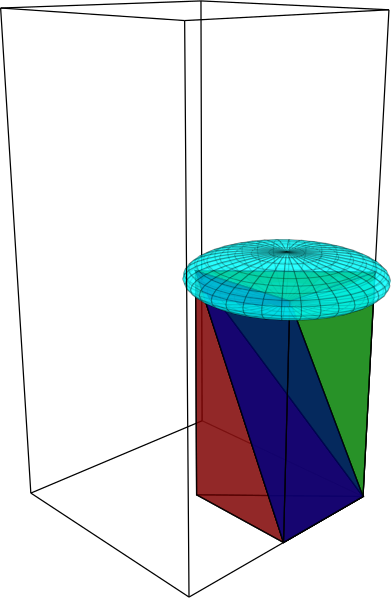
\includegraphics[height=2.5cm]{d3c3_2_splitting1.pdf}
	  \end{figure}
	\item $E^2$-type splitting: \mode<presentation>{"cut along tori"}
	  \mode<article>{In Thurston-conjecture "cut along tori". This indicates
	  two parts in the tiling, in both parts the other part can be seen as
	  an ideal vertex. There are at least 3 possible combinations, from
	  which only the first one indicates a splitting, the second one most
	  likely indicates a fibration and the third one is not possible,
	  because inside the torus there is a full $2$-dimensional plane. (See
	  fig. \ref{fig:e2splitting}.)}
	  \begin{figure}
	    \mode<article>{\caption{\label{fig:e2splitting} $E^2$-type splittings}}
	    \center
	    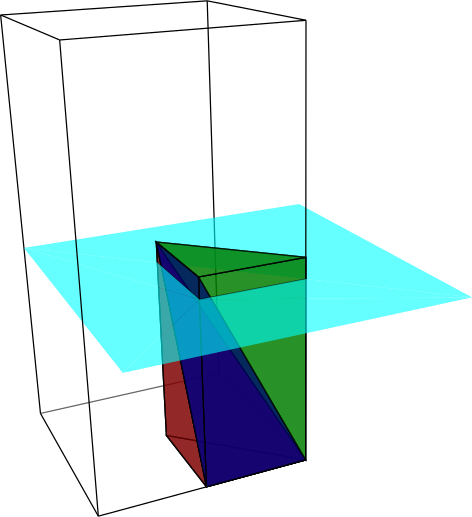
\includegraphics[height=2.5cm]{d3c3_2_splitting2_alt1.pdf}
	    \hspace{0.1\textwidth}
	    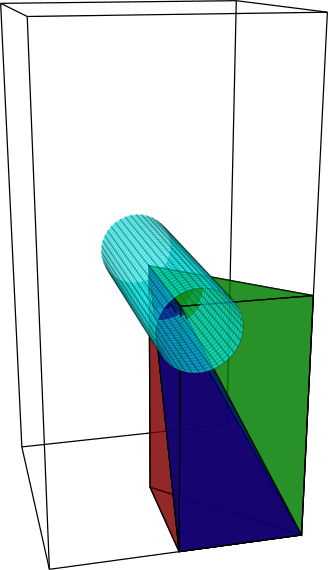
\includegraphics[height=2.5cm]{d3c3_2_splitting2_alt2.pdf}
	    \hspace{0.1\textwidth}
	    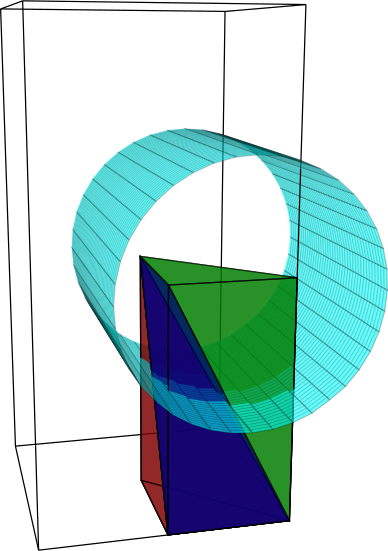
\includegraphics[height=2.5cm]{d3c3_2_splitting2.pdf}
	  \end{figure}
      \end{itemize}
    \item Find out the signature of the projective space\mode<article>{ with a
      nice large library of articles.}
  \end{itemize}
\end{frame}
  \begin{itemize}
    \item $S^2$-type splitting: Indicates a detail in the tiling, which is
      shrinkable to a single vertex, so we get a similar tiling \mode<article>{ with
      less simplex-vertices, so} with less simplex-orbits. (Possible bad
      orbifold problem.) \mode<article>{(See fig. \ref{fig:s2splitting}.)}
    \item $E^2$-type splitting: In Thurston-conjecture "cut along tori". This
      indicates two parts in the tiling, in both parts the other part
      can be seen as an ideal vertex. \mode<article>{There are at least 3
      possible combinations, from which only the first one indicates a
      splitting, the second one most likely indicates a fibration and the third one
      is not possible, because inside the torus there is a full $2$-dimensional
      plane. (See fig. \ref{fig:e2splitting}.)}
  \end{itemize}                      

\begin{frame}
  \nocite{DHM93,D87,Du88,H93,LM90,Ma67,M94,T82,VS93,F94,F03}
  \bibliographystyle{plain}
  \mode<presentation>{\fontsize{5pt}{0}}
  \bibliography{dsym}
\end{frame}

\begin{frame}
  \frametitle{Questions?}
  \center\large Questions?
\end{frame}

\end{document}
